\section{Answer to Question \ref{q:why}: The cause of clusterization}\label{section:why}
\begin{figure}
    \centering
    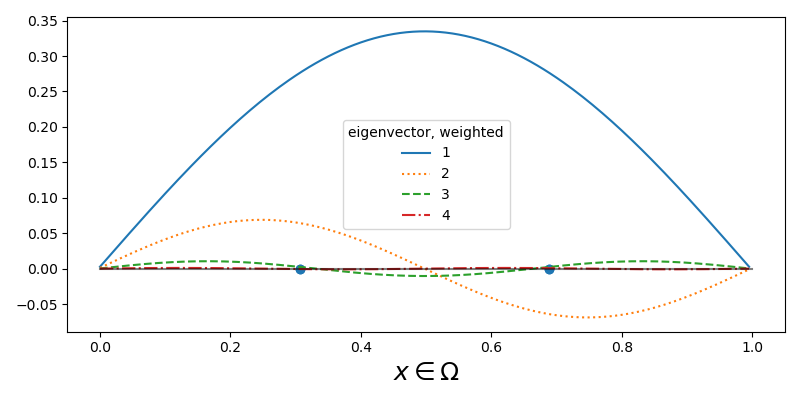
\includegraphics[height=0.5\textwidth]{eigenvectors.pdf}
    \caption{D-optimal measurement locations ($m=5$ measurements) and
      weighted eigenvectors for inversion of the initial condition of
      the 1D heat equation. Measurement locations and weighted
      eigenvectors are plotted over the computational domain $\Omega =
      [0, 1]$ (x-axis). Measurement clusterization occurs
      approximately at $0.31$ and $0.69$. These two locations are a
      compromise between zeros of eigenvectors a D-optimal design aims
      to ignore (third and up) and staying far from a zero of the
      first and second eigenvectors. Allocating $m=5$ measurements
      into two locations results in clusterization, according to the
      pigeonhole principle.}
  \label{fig:why}
\end{figure}


According to Theorem \ref{thm:char}, D-optimal designs aim to capture
a small subset of eigenvectors of the prior covariance, specifically
the $k$ eigenvectors with the highest prior variance. Our model
naturally achieves this objective by not measuring eigenvectors $k+1$
and above, as proven in Theorem \ref{thm:char}. Translating this
understanding to spatial problems, we anticipate that a D-optimal
design would favor measurement locations where eigenvectors $k+1$ and
above are either close to zero in value or possess small eigenvalues
in the prior spectrum, for some $k > 0$. To illustrate this
preference, Figure \ref{fig:why} depicts the scenario using the 1D
heat equation with homogeneous Dirichlet boundary conditions (details
in the supplementary material). The plot showcases four eigenvectors,
scaled according to their prior standard deviations. Since
eigenvectors beyond the fourth have insignificant prior eigenvalues,
we exclude them from consideration. Notably, we observe that
measurements are clustered near the zeros of the third and fourth
eigenvectors, so we conclude that $k=2$. Clusterization arises because
there are only two locations where the third and fourth eigenvectors
approach zero, while the first and second eigenvectors exhibit
significantly non-zero values. Consequently, when we allocate four
measurements to these two locations, they naturally cluster together,
aligning with the pigeonhole principle.
